%%%%%%%%%%%%%%%%%%%%%%%%%%%%%%%%%%%%%%%%%%%%%%%%%%%%%%%%%%%%%%%%%%%%%
%                                                                   %
%	CHAPTER ONE, CHOICES AND SPH                                    %
%                                                                   %
%%%%%%%%%%%%%%%%%%%%%%%%%%%%%%%%%%%%%%%%%%%%%%%%%%%%%%%%%%%%%%%%%%%%%
\chapter{Complex system modelization}

\section{Introduction}
In this chapter we give details on our choice for the generic application which is confronted to both computation and communication walls in irregular context. 
The problem we choose, the Smoothed Particle Hydrodynamics simulation method, is described on a physical aspect.
We point out the difficulties involved in the implementation on supercomputers and especially hybrid architectures.  
A lot of work have been spent on the comprehension of the physical aspects to produce a code that meet the behavior of real astrophysics simulations.

The first section is a presentation of the SPH method itself and the overall limitation we face. 
Then we describe different kind of specific simulations we use as a benchmark of the application itself. 

\section{Physical modelization and downsides}
We identified two main walls in our metrics:
The computational wall and the communication/memory one.
We conducted tests on both aspects keeping the irregularity behavior as a good representative of production codes.
We show how these requirements are meet in the same problem with SPH and gravitation.
In order to add another complexity layer in term of irregularity for both computation and communication we targeted astrophysical simulations. 
They require the computation of gravitation in addition to SPH on a very high number of particles. 
This part describes the SPH method itself and the gravitation computation based on fast multipole methods. 

\subsection{Smoothed Particles Hydrodynamics}
\label{sec:intro_sph}
Smoothed Particle Hydrodynamics (SPH) is an explicit numerical mesh-free Lagrangian method.
It is used to solve hydrodynamical partial differential equations (PDEs)\index{Partial Differential Equations} by discretized them into a set of fluid elements called particles. 
This computational method was invented for the purpose of astrophysics simulations by Monaghan, Gingold and Lucy in 1977 \cite{lucy1977numerical,gingold1977smoothed}. 
This first SPH work conserved mass and they later proposed a method which also conserves linear and angular momenta \cite{gingold1982kernel}. 
The method was extended for general fluid simulations and many more fields from ballistics to oceanography.
The development of new reliable, parallel and distributed tools for this method is a challenge for future HPC architectures with the upcoming exascale systems.

%
\begin{figure}
\centering
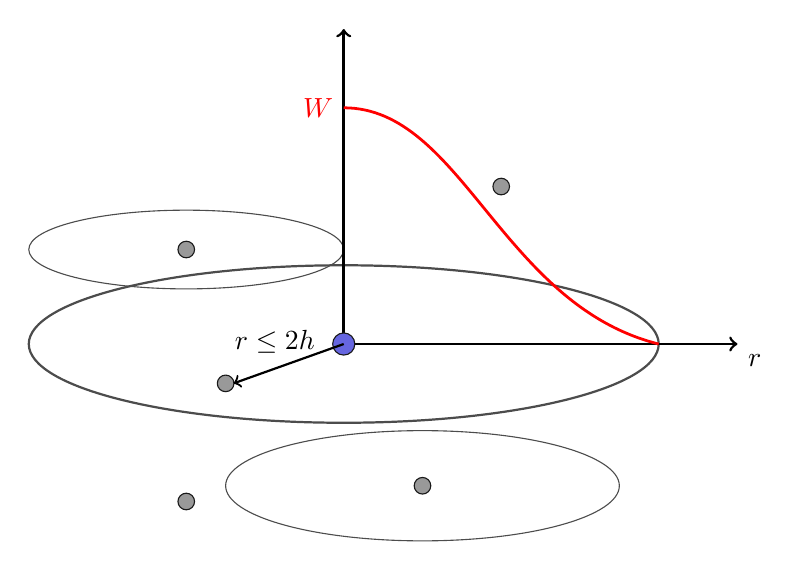
\begin{tikzpicture}
	
	% Others and their ellipse
	\draw [black!90,fill=black!40] (.5,1.5) circle (.3em);
	\draw [black!90,fill=black!40] (0,0) circle (.3em);
	\draw [black!90,fill=black!40] (0,3.2) circle (.3em);
	\draw[black!70] (0,3.2) ellipse (2 and .5);
	\draw [black!90,fill=black!40] (3,.2) circle (.3em);
	\draw[black!70] (3,.2) ellipse (2.5 and .7);
	\draw [black!90,fill=black!40] (4,4) circle (.3em);
	% Ellipses 
	\draw[line width=.8pt,black!70] (2,2) ellipse (4 and 1);
	% Axes
	\draw[->,line width=1pt] (2,2) -- (7,2) node[anchor=north west] {$r$};
	\draw[->,line width=1pt] (2,2) -- (2,6);
	% bezier for kernel 
	\draw[red,line width=1pt]  (6,2) .. controls (4,2.5) and (3.5,5) .. (2,5) node[red,anchor=east] {$W$};
	% main particle, at the end to cover
	\draw [black!90,fill=black!20!blue!60] (2,2) circle (.4em);
	% Arrows 
	\draw[->,line width=.8pt] (2,2) -- (.6,1.5) node[midway, above,xshift=-.5em] {$r\leq2h$};
\end{tikzpicture}
%\includegraphics[scale=.4]{\locpath/figures/flecsph/sph.pdf}
\caption{SPH kernel $W$ and smoothing length $h$ representation}
\label{fig:sph_base}
\end{figure}
%
The method, as illustrated in figure~\ref{fig:sph_base}, computes the evolution of a group of particles representing physical quantities.
Those physical quantities are either invariant or computed for every particle at each step regarding its neighbors in the radius of its smoothing length $h$. 
The particles in this radius are then valued according to their distance using a smoothing function $W$, also called a kernel\index{Smoothing Kernel}. 
The fundamental SPH formulation for any physical quantity $A$ is then, with all the neighbors $b$ of a particle $a$:
\begin{equation}
A(\vec{r})_a \simeq \sum_b \frac{m_b}{\rho_b} A(\vec{r}_b) W ( |\vec{r}-\vec{r}_b|,h)
\end{equation}

On a physics aspect, this method has several advantages:
it can handle deformations, low densities, vacuum, and makes particle tracking easier. 
It also conserves mass, linear and angular momenta, and energy by its construction that implies independence of the numerical resolution. 
Another strong benefit of using SPH is its exact advection of fluid properties. 
Furthermore, the particle structure of SPH easily combines with tree methods for solving Newtonian gravity through N-body simulations.
As a mesh-free method, it avoids the need of grid to calculate the spatial derivatives. 

However, there are cons to consider using SPH: 
it cannot be extend to all PDE formulations;
it requires careful setup of initial distribution of particles; 
further, it can be struggle to resolve turbulence-dominated flows and special care must be taken when handling high gradients such as shocks and surface structure of neutron stars.
Many works are leading to handle more cases and to push the limitations of this method \cite{dai2017dual,lind2016incompressible,ren2016dual}.\\

In this work, we are solving Lagrangian conservation equations (Euler equations) for density, energy and momentum of an ideal fluid ~\cite{Landau1959}  such that:
\begin{equation}
\frac{d \rho}{d t} = - \rho ( \nabla \cdot \vec{v}), \quad
\frac{d u}{d t} = - \frac{P}{\rho} ( \nabla \cdot \vec{v} ), \quad
\frac{d \vec{v}}{d t} = - \frac{1}{\rho} (\nabla P)
\end{equation}
with $\rho$ the density, $P$ the pressure, $u$ the internal energy and $v$ the velocity, $\nabla$ the nabla operator and where $d/dt = \partial/\partial_t + \vec{v} \cdot \nabla$ which is convective derivative.

By using the volume element $V_b = m_b / \rho_b$, we can formulate the Newtonian SPH scheme~\cite{rosswog2009} such that
\begin{equation}
\label{eq:rho}
\rho_a = \sum_b m_b W_{ab} (h_a)
\end{equation}
\begin{equation}
\frac{d u_a}{dt} = \frac{P_a}{\rho_a^2} \sum_b m_b \vec{v}_{ab} \cdot \nabla_a W_{ab} 
\end{equation}
\begin{equation}
\frac{d \vec{v}_a}{d t} = - \sum_b m_b \left(\frac{P_a}{\rho_a^2} + \frac{P_b}{\rho_b^2} \right) \nabla_a W_{ab}
\end{equation}
where $W_{ab} = W(| \vec{r}_a - \vec{r}_b |,h)$ is the smoothing kernel. 
The equations we would like to solve allow for emergence of discontinuities from smooth initial data. 
At discontinuities, the entropy increases in shocks. That dissipation occurs inside the shock-front. 
The SPH formulation here is inviscid so we need to handle this dissipation near shocks. 
There are a number of way to handle this problem, but the most widespread approach is to add artificial viscosity (or artificial dissipation) terms in SPH formulation such that:
\begin{equation}
\left(\frac{d u_a}{dt} \right)_{art} = \frac{1}{2} \sum_b m_b \Pi_{ab} \vec{v}_{ab} \cdot \nabla_a W_{ab}
\end{equation}
\begin{equation}
\left(\frac{d\vec{v}_a}{dt} \right)_{art} = - \sum_b m_b \Pi_{ab}\nabla_a W_{ab}
\end{equation}
In general, we can express the equations for internal energy and acceleration with artificial viscosity
\begin{equation}
\label{eq:intern}
\frac{d u_a}{dt} = \sum_b m_b \left(\frac{P_a}{\rho_a^2} + \frac{\Pi_{ab}}{2} \right) \vec{v}_{ab} \cdot \nabla_a W_{ab}
\end{equation}
\begin{equation}
\label{eq:velo}
\frac{d \vec{v}_a}{d t} = - \sum_b m_b \left(\frac{P_a}{\rho_a^2} + \frac{P_b}{\rho_b^2} + \Pi_{ab} \right) \nabla_a W_{ab}
\end{equation}
$\Pi_{ab}$ is the artificial viscosity tensor. 
As long as $\Pi_{ab}$ is symmetric, the conservation of energy, linear and angular momentum is assured by the form of the equation and antisymmetry of the gradient of kernel with respect to the exchange of indices $a$ and $b$. $\Pi_{ab}$ may define in different ways and here we use~\cite{Monaghan1983} such as: 
\begin{equation}
\Pi_{ab} = \begin{cases}
\frac{- \alpha \bar{c}_{ab} \mu_{ab} + \beta \mu_{ab}^2}{\bar{\rho}_{ab}} & \text{for $\vec{r}_{ab} \cdot \vec{v}_{ab} < 0$} \\
0 & \text{otherwise}
\end{cases}
\end{equation}
\begin{equation}
\mu_{ab} = \frac{\bar{h}_{ab} \vec{r}_{ab} \cdot \vec{v}_{ab}}{r^2_{ab} + \epsilon \bar{h}_{ab}^2}
\end{equation}

Using the usual form $c_s$ as $c_s = \sqrt{\frac{\partial p}{\partial \rho}}$.
The values of $\epsilon$, $\alpha$, and $\beta$ have to be set regarding the problem targeted. 
As an example we used for the Sod shock tube problem: $\epsilon = 0.01h^2$, $\alpha = 1.0$, and $\beta = 2.0$. 


There are many possibilities for the smoothing function, called the kernel. 
As an example the Monaghan's cubic spline kernel is given by:
\begin{equation}
W(\vec{r_{ij}},h) = \frac{\sigma}{h^D} \begin{cases}
1-\frac{3}{2} q^2 + \frac{3}{4} q^3 & \text{if} \indent 0 \leq q \leq 1 \\
\frac{1}{4} (2-q)^3  & \text{if} \indent 1 \leq q \leq 2 \\
0 & \text{otherwise}
\end{cases}
\end{equation}
where $q = r/h$, $r$ the distance between the two particles, $D$ is the number of dimensions and $\sigma$ is a normalization constant with the values:
\begin{equation}
\sigma =  \begin{cases}
\frac{2}{3} & \text{for 1D}  \\
\frac{10}{7 \pi} & \text{for 2D} \\
\frac{1}{\pi} & \text{for 3D}
\end{cases}
\end{equation}

In the computation of forces we also need to apply the gradient of the smoothing kernel. 
This is, in our example, for the cubic spline kernel:
\begin{equation}
 \vec{\nabla}_iW(\vec{r_{ij}},h) = \frac{\sigma}{h^{D+1}} \times \begin{cases} ( -\frac{3}{h} + \frac{9}{4h}q) \vec{r_{ij}}, & \mbox{si } 0 \leq \frac{r}{h} < 1 \\ (\frac{-3}{r} + \frac{3}{h} - \frac{3}{4h}q ) \vec{r_{ij}}, & \mbox{si } 1 \leq \frac{r}{h} < 2\\ 0, & \mbox{si } \frac{r}{h} \geq 2 \end{cases}
\end{equation}

\begin{figure}[t!]
\centering
\begin{tikzpicture}
	\draw[->] (-7,0) -- (7,0) node[right] {$r$};
    \draw[->] (0,0) -- (0,2.5) node[above] {$W$};

    \foreach \v in {-3,-2,...,2,3}{
	   \draw (\v*2,.1) -- (\v*2,-.1) node[below] {\v};
    }

    \draw (-.1,2) -- (.1,2) node [above right] {1};

    \draw[very thick,scale=2,domain=0:1,smooth,variable=\r,blue] plot ({\r},{1-(3/2*\r*\r)+(3/4*\r*\r*\r)});
    \draw[very thick,scale=2,domain=0:1,smooth,variable=\r,blue] plot ({-\r},{1-(3/2*\r*\r)+(3/4*\r*\r*\r)});

    \draw[very thick, scale=2,domain=1:2,smooth,variable=\r,blue] plot ({\r},{1/4*(2-\r)*(2-\r)*(2-\r)});
    \draw[very thick, scale=2,domain=1:2,smooth,variable=\r,blue] plot ({-\r},{1/4*(2-\r)*(2-\r)*(2-\r)});

    \draw[very thick,scale=2,domain=2:3,smooth,variable=\r,red] plot ({\r},{0});
    \draw[very thick,scale=2,domain=2:3,smooth,variable=\r,red] plot ({-\r},{0});
\end{tikzpicture}
\caption{Cubic spline kernel example with $\sigma = 1$ and $h = 1$}
\label{fig:cubic_spline_function}
\end{figure}

Figure~\ref{fig:cubic_spline_function} is a representation of the cubic spline kernel with $\sigma = 1$ and $h = 1$. 
The abscissa axis represent $r$, distance between the particles and the ordinate the value of the smoothing kernel.
When the support of the function, $2$ is reached the particles are ignored $W=0$, represented in red on the figure. 

To sum up, the SPH resolution scheme and its routines are presented on algorithm \ref{alg:sph}.
The Equation of State (EOS) and the integration are problem dependent and will be define for each test case in section \ref{sec:applications}. 

\begin{algorithm}
\caption{SPH loop algorithm}\label{alg:sph}
\begin{algorithmic}[1]
\While{not last step}
\State Compute density for each particle (\ref{eq:rho})
\State Compute pressure using EOS 
\State Compute acceleration from pressure forces (\ref{eq:velo})
\State Compute change of internal energy for acceleration (\ref{eq:intern})
\State Advance particles after integration
\EndWhile
\end{algorithmic}
\end{algorithm}

The main downside for the implementation of this method is the requirement for local computation on every particle. 
The particles have to be grouped locally to perform the computation of (\ref{eq:rho}), (\ref{eq:intern}) and (\ref{eq:velo}).
A communication step is needed before and after (\ref{eq:rho}) to get the local physical data to be able to compute (\ref{eq:intern}) and (\ref{eq:velo}).
The tree data structure allows us to perform $O(Nlog(N))$ neighbor search but also add a domain decomposition and distribution layer.

\subsection{Gravitation}
In order to target hard irregular simulation facing both the communication and computation wall in irregular behavior we decided to simulate astrophysical events. 
This choice is also accurate since our code, FleCSPH, will be use by the LANL astrophysicists in the near future. 
In order to perform those simulation the computation of gravitation/self-gravitation is required. 
This part present our implementation choice and expose the main problems for HPC implementation. 


For classical problems like fluid flow the gravitation can directly be applied on the particles with the force:
\begin{equation}
	\vec{a_g} = m\vec{g}
\end{equation}

In order to consider astrophysics problems we need to introduce self-gravitation and gravitation. 
Each particle imply an action on the others based on its distance and mass. 
The equation of gravitation for a particle $i$ with $j$ other particles is: 
\begin{equation}
	\vec{f_a}_i = \sum_j -G \frac{m_i m_j}{|\vec{r_i}-\vec{r_j}|^3} \vec{r_{ij}}
	\label{eq:gravitation}
\end{equation}

This computation involve an $O(N^2)$ complexity and thus is not applicable directly. 
We applied the method called Fast Multipole Method, FMM and discussed in \cite{beatson1997short}.
This method is perfectly adapted to a tree representation of the domain and particles. 

\begin{figure}[ht!]
\resizebox {\columnwidth} {!} {
\begin{tikzpicture}
\def\nrand{300}
\def\seed{12}
\def\gridSize{5mm}
\def\gridTotal{4}
% Particles to Multipole
\pgfmathsetseed{\seed}
\begin{scope}[
   		yshift=0,every node/.append style={
    		yslant=0.5,xslant=-1},yslant=0.5,xslant=-1
    ]
    \fill[white,fill opacity=.9] (0,0) rectangle (4,4);
    \draw[black,very thick] (0,0) rectangle (4,4);
	\draw[step=\gridSize, black] (0,0) grid (\gridTotal,\gridTotal);
	\foreach \i in {1,2,...,\nrand}{
    	\pgfmathsetmacro{\x}{(rand)*2+2}
    	\pgfmathsetmacro{\y}{(rand)*2+2}
		% COLOR 
		\ifthenelse{\( \lengthtest{\x cm>2cm} \AND \lengthtest{\x cm<2.5cm} \)}
		{	
			\ifthenelse{ \( \lengthtest{\y cm>1cm} \AND \lengthtest{\y cm<1.5cm} \)}
			{\node at (\x,\y) [black!50!green,circle,fill,inner sep=.7pt,minimum size=3pt]{};}
			{\node at (\x,\y) [circle,fill,inner sep=.7pt]{};}
		}
		{\node at (\x,\y) [circle,fill,inner sep=.7pt]{};}
	}
\end{scope}
\pgfmathsetseed{\seed}
\begin{scope}[
   		yshift=80,every node/.append style={
    		yslant=0.5,xslant=-1},yslant=0.5,xslant=-1
    ]
    \fill[white,fill opacity=.9] (0,0) rectangle (4,4);
    \draw[black,very thick] (0,0) rectangle (4,4);
	\draw[step=5mm, black] (0,0) grid (\gridTotal,\gridTotal);
	\foreach \x in {0,1,...,7}{\foreach \y in {0,1,...,7}{
		\ifthenelse{\( \x<3 \OR \x>5 \)}
		{
			\node at (\x*\gridSize+\gridSize/2,\y*\gridSize+\gridSize/2)[red,circle,fill,inner sep=.7pt,minimum size=3pt]{};
		}
		{	\ifthenelse{ \( \y<1 \OR \y>3 \)}
			{
			\node at (\x*\gridSize+\gridSize/2,\y*\gridSize+\gridSize/2)[red,circle,fill,inner sep=.7pt,minimum size=3pt]{};	
			}{}
		}
	}}
	\foreach \i in {1,2,...,\nrand}{
    	\pgfmathsetmacro{\x}{(rand)*2+2}
    	\pgfmathsetmacro{\y}{(rand)*2+2}
    	\ifthenelse{\( \lengthtest{\x cm<1.5cm} \OR \lengthtest{\x cm>3cm} \)}
		{\node at (\x,\y) [blue,circle,fill,inner sep=.7pt]{};}
		{	\ifthenelse{ \( \lengthtest{\y cm<.5cm} \OR \lengthtest{\y cm>2cm} \)}
			{\node at (\x,\y) [blue,circle,fill,inner sep=.7pt]{};}
			{}
		}
  	}
\end{scope}
\begin{scope}[
   		yshift=160,every node/.append style={
    		yslant=0.5,xslant=-1},yslant=0.5,xslant=-1
    ]
    \fill[white,fill opacity=.9] (0,0) rectangle (4,4);
    \draw[black,very thick] (0,0) rectangle (4,4);
	\draw[step=10mm, black] (0,0) grid (4,4);
	\foreach \x in {0,1}{\foreach \y in {0,...,7}{
		\node at (\x*\gridSize+\gridSize/2,\y*\gridSize+\gridSize/2)[blue,circle,fill,inner sep=.7pt]{};
	}}
	\foreach \x in {0,...,7}{\foreach \y in {6,7}{
		\node at (\x*\gridSize+\gridSize/2,\y*\gridSize+\gridSize/2)[blue,circle,fill,inner sep=.7pt]{};
	}}

	\foreach \x in {0}{\foreach \y in {0,...,3}{				  
		\node at (\x*\gridSize*2+\gridSize,\y*\gridSize*2+\gridSize) [red,circle,fill,inner sep=.7pt,minimum size=3pt]{};
	}}
	\foreach \x in {0,...,3}{\foreach \y in {3}{				  
		\node at (\x*\gridSize*2+\gridSize,\y*\gridSize*2+\gridSize) [red,circle,fill,inner sep=.7pt,minimum size=3pt]{};
	}}
\end{scope}

%PARTICLES TO PARTICLES
\pgfmathsetseed{\seed}
\begin{scope}[
   		yshift=0,xshift=9cm,every node/.append style={
    		yslant=0.5,xslant=-1},yslant=0.5,xslant=-1
    ]
    \fill[white,fill opacity=.9] (0,0) rectangle (4,4);
    \draw[black,very thick] (0,0) rectangle (4,4);
	\draw[step=5mm, black] (0,0) grid (4,4);
	\foreach \i in {1,2,...,\nrand}{
    	\pgfmathsetmacro{\x}{(rand)*2+2}
    	\pgfmathsetmacro{\y}{(rand)*2+2}
    	\ifthenelse{\( \lengthtest{\x cm>1.5cm} \AND \lengthtest{\x cm<3cm} \)}
		{	
			\ifthenelse{ \( \lengthtest{\y cm>.5cm} \AND \lengthtest{\y cm<2cm} \)}
			{
				% COLOR 
				\ifthenelse{\( \lengthtest{\x cm>2cm} \AND \lengthtest{\x cm<2.5cm} \)}
				{	
					\ifthenelse{ \( \lengthtest{\y cm>1cm} \AND \lengthtest{\y cm<1.5cm} \)}
					{\node at (\x,\y) [red,circle,fill,inner sep=.7pt,minimum size=3pt]{};}
					{\node at (\x,\y) [blue,circle,fill,inner sep=.7pt]{};}
				}
				{\node at (\x,\y) [blue,circle,fill,inner sep=.7pt]{};}
			}{}
		}{}
    	%\node at (\x,\y) [circle,fill,inner sep=.7pt]{};
  	}
\end{scope}
%MULTIPOLE TO MULTIPOLE
\begin{scope}[
   		yshift=160,xshift=9cm,every node/.append style={
    		yslant=0.5,xslant=-1},yslant=0.5,xslant=-1
    ]
    \fill[white,fill opacity=.9] (0,0) rectangle (4,4);
    \draw[black,very thick] (0,0) rectangle (4,4);
    \draw[step=10mm, black] (0,3) grid (4,4);
	\draw[step=10mm, black] (0,0) grid (1,3);
	\draw[step=5mm, black] (1,0) grid (2,3);
	\draw[step=5mm, black] (2,2) grid (4,3);
	\draw[step=5mm, black] (2,0) grid (4,.5);
	\draw[step=5mm, black] (3.5,0) grid (4,2);
	% add rectangle
	\draw[black] (2,.5) rectangle (3.5,2);
	% Big part 
	\foreach \x in {0}{\foreach \y in {0,...,3}{				  
		\node at (\x*\gridSize*2+\gridSize,\y*\gridSize*2+\gridSize) [blue,circle,fill,inner sep=.7pt]{};
	}}
	\foreach \x in {0,...,3}{\foreach \y in {3}{				  
		\node at (\x*\gridSize*2+\gridSize,\y*\gridSize*2+\gridSize) [blue,circle,fill,inner sep=.7pt]{};
	}}
	% Smaller one 
	\foreach \x in {2,3}{\foreach \y in {0,...,3}{
		\node at (\x*\gridSize+\gridSize/2,\y*\gridSize+\gridSize/2)[blue,circle,fill,inner sep=.7pt]{};
	}}

	\foreach \x in {2,...,7}{\foreach \y in {4,5}{
		\node at (\x*\gridSize+\gridSize/2,\y*\gridSize+\gridSize/2)[blue,circle,fill,inner sep=.7pt]{};
	}}

	\foreach \x in {7}{\foreach \y in {0,...,3}{
		\node at (\x*\gridSize+\gridSize/2,\y*\gridSize+\gridSize/2)[blue,circle,fill,inner sep=.7pt]{};
	}}
	\foreach \x in {4,5,6}{\foreach \y in {0}{
		\node at (\x*\gridSize+\gridSize/2,\y*\gridSize+\gridSize/2)[blue,circle,fill,inner sep=.7pt]{};
	}}
	\node at (5*\gridSize+\gridSize/2,2*\gridSize+\gridSize/2) [red,circle,fill,inner sep=.7pt,minimum size=3pt]{};
\end{scope}

% Multipole to Particles 
\pgfmathsetseed{\seed}
\begin{scope}[
   		yshift=0,xshift=18cm,every node/.append style={
    		yslant=0.5,xslant=-1},yslant=0.5,xslant=-1
    ]
    \fill[white,fill opacity=.9] (0,0) rectangle (4,4);
    \draw[black,very thick] (0,0) rectangle (4,4);
	\draw[step=5mm, black] (0,0) grid (4,4);
	\foreach \i in {1,2,...,\nrand}{
    	\pgfmathsetmacro{\x}{(rand)*2+2}
    	\pgfmathsetmacro{\y}{(rand)*2+2}
		% COLOR 
		\ifthenelse{\( \lengthtest{\x cm>2cm} \AND \lengthtest{\x cm<2.5cm} \)}
		{	
			\ifthenelse{ \( \lengthtest{\y cm>1cm} \AND \lengthtest{\y cm<1.5cm} \)}
			{\node at (\x,\y) [black!50!green,circle,fill,inner sep=.7pt,minimum size=3pt]{};}
			{\node at (\x,\y) [circle,fill,inner sep=.7pt]{};}
		}
		{\node at (\x,\y) [circle,fill,inner sep=.7pt]{};}
	}
\end{scope}
\pgfmathsetseed{\seed}
\begin{scope}[
   		yshift=80,xshift=18cm,every node/.append style={
    		yslant=0.5,xslant=-1},yslant=0.5,xslant=-1
    ]
    \fill[white,fill opacity=.9] (0,0) rectangle (4,4);
    \draw[black,very thick] (0,0) rectangle (4,4);
	\draw[step=5mm, black] (0,0) grid (4,4);

	\foreach \i in {1,2,...,\nrand}{
    	\pgfmathsetmacro{\x}{(rand)*2+2}
    	\pgfmathsetmacro{\y}{(rand)*2+2}
    	\ifthenelse{\( \lengthtest{\x cm>1.5cm} \AND \lengthtest{\x cm<3cm} \)}
		{	
			\ifthenelse{ \( \lengthtest{\y cm>.5cm} \AND \lengthtest{\y cm<2cm} \)}
			{
				% COLOR 
				\ifthenelse{\( \lengthtest{\x cm>2cm} \AND \lengthtest{\x cm<2.5cm} \)}
				{	
					\ifthenelse{ \( \lengthtest{\y cm>1cm} \AND \lengthtest{\y cm<1.5cm} \)}
					{\node at (\x,\y) [red,circle,fill,inner sep=.7pt,minimum size=3pt]{};}
					{}
				}{}
			}{}
		}{}
	}
	\node at (4*\gridSize+\gridSize/2,2*\gridSize+\gridSize/2) [blue,circle,fill,inner sep=.7pt]{};
\end{scope}
%% MULTIPOLE TO LOCAL
\begin{scope}[
   		yshift=160,xshift=18cm,every node/.append style={
    		yslant=0.5,xslant=-1},yslant=0.5,xslant=-1
    ]
    \fill[white,fill opacity=.9] (0,0) rectangle (4,4);
    \draw[black,very thick] (0,0) rectangle (4,4);
	\draw[step=5mm, black] (0,0) grid (4,4);
	\node at (4*\gridSize+\gridSize/2,2*\gridSize+\gridSize/2) [red,circle,fill,inner sep=.7pt,minimum size=3pt]{};

	\node at (5*\gridSize+\gridSize/2,2*\gridSize+\gridSize/2) [blue,circle,fill,inner sep=.7pt]{};
\end{scope}
% ARROWS AND TEXT
\draw[->,very thick] (-3,2.8) -- (-3,4) node[midway,left] {\textbf{P2M}};
\draw[->,very thick] ([yshift=80]-3,2.8) -- ([yshift=80]-3,4) node[midway,left] {\textbf{M2M}};

\draw[->,very thick] ([yshift=160]3,2.8) -- ([yshift=160]6,2.8) node[midway,above] {\textbf{M2L}};
\draw[->,very thick] ([yshift=160,xshift=9cm]3,2.8) -- ([yshift=160,xshift=9cm]6,2.8) node[midway,above] {\textbf{L2L}};

\draw[<-,very thick] ([yshift=80]21,2.8) -- ([yshift=80]21,4) node[midway,right] {\textbf{L2P}};
\draw[<-,very thick] (21,2.8) -- (21,4) node[midway,right] {\textbf{SUM}};

\draw[->,very thick] (3,2.8) -- (6,2.8) node[midway,above] {\textbf{P2P}};
\draw[->,very thick] ([xshift=9cm]3,2.8) -- ([xshift=9cm]6,2.8) node[midway,above] {\textbf{SUM}};


\draw[->,very thick] (-3.5,8.7cm) node[xshift=-5pt,blue,circle,fill,inner sep=.7pt,minimum size=3pt] (a) {} -- 
 (-3,8.7cm) node[xshift=5pt,red,circle,fill,inner sep=.7pt,minimum size=3pt] (b) {};
\node[align=left] at (-3,9.5cm) {Data\\direction};


\end{tikzpicture}
}
\caption{Fast Multipole Method schematics. Particles to Multipole (P2M), Multipole to Multipole (M2M), Multipole to Particles (M2P), Multipole to Local (M2L), Local to Local (L2L) and Particles to Particles (P2P). Schematic inspired from \cite{yokota2011treecode}}
\label{fig:gravitation_fmm}
\end{figure}

This method aim to compute the gravitation up to an approximation determined by the user. 
Details are given in figure~\ref{fig:gravitation_fmm}, from left bottom to right bottom for a group of particles.
We identify three main actors in this method: \\

\begin{description}[noitemsep,nolistsep]
\item[Particles: ] the bodies on which we need to compute the gravitation regarding the other particles. 
In figure~\ref{fig:gravitation_fmm} we separate the green particles, on which we are computing the gravitation, from the other, blue, particles. 
\item[Multipoles: ] the center of mass for a group of particles.
In our example they regroup the mass and barycenter of the sub-particles. 
There are several level of multipoles: particles' multipole and multipoles' multipole.
\item[Locals: ] the center of mass for the reduction on the particles concerned in this walk. 
They have the same behavior as the multipoles but the information goes down to particles instead of up.\\ 
\end{description}

In order to compute the gravitation for a group of particles in the domain the steps are: \\

\begin{description}[noitemsep,nolistsep]
	\item[Particles to Particles (P2P): ] For the particles that are close, use the direct $O(N^2)$ algorithm.  
	This is the part that grow if the user desires more accurate results. 
	\item[Particles to Multipoles (P2M): ] Gather the data of all the sub-particles to the centers of mass, the multipoles.
	This is the first layer of the tree, the leaves. 
	\item[Multipoles to Multipole (M2M): ] Gather the data of multipoles on higher level of the tree from the leaves to the root. 
	\item[Multipoles to Local (M2L): ] Compute the gravitation part of all the distant multipole to the local. 
	\item[Local to Local (L2L): ] Go down in the tree and spread the component to sub-locals.
	\item[Local to Particles (L2P): ] When a leaf of the tree is reached, compute the application of the local for all sub-particles. 
	\item[Summation: ] At the end of the computation for both P2P and L2P the two interactions can be summed up to compute the gravitation applied to the particles. \\
\end{description}

This scheme have to be repeat for every group of particles. 
The P2M-M2M steps are done just once before the FMM method for all the groups of particles.
For the choice between either P2P or M2L we use a criterion call MAC, Multipole Acceptance Criterion. 	
In this study we used an angle between the local center of mass and the edge of distant multipole. 
If the angle fits the criterion we use the current multipole, otherwise we go lower in the tree to consider smaller multipole.
If the criterion never match, we are too close and consider P2P.\\

For the P2P step, the classical gravitation computation is used, like presented in equation~\ref{eq:gravitation}.
But for the interaction with distant multipoles, we use a Taylor series.\\
The gravitation function of equation~\ref{eq:gravitation} can be approximate on a particle at position $\vec{r}$ by the gravitation computed at the centroid at position $\vec{r_c}$: 
\begin{equation}
\label{eq:taylor_series}
 \vec{f}(\vec{r}) = \vec{f}(\vec{r_c}) + ||\frac{\partial\vec{f}}{\partial\vec{r}}||\cdot (\vec{r} - \vec{r_c}) + \frac{1}{2} (\vec{r}-\vec{r_c})^\intercal \cdot   ||\frac{\partial\vec{f}}{\partial\vec{r} \partial\vec{r}}|| \cdot (\vec{r} - \vec{r_c})
 \end{equation}

 From equation~\ref{eq:gravitation} we compute the term $||\frac{\partial\vec{f}}{\partial\vec{r}}||$:
 \begin{equation}
\frac{\partial\vec{f}}{\partial\vec{r}} =
- \sum_p \frac{m_p}{|\vec{r_c}-\vec{r_p}|^3}
\begin{bmatrix}
1 - \frac{3(x_c-x_p)(x_c-x_p)}{|\overline{r_c}-\overline{r_p}|^2} & -\frac{3(y_c-y_p)(x_c-x_p)}{|\overline{r_c}-\overline{r_p}|^2}  & -\frac{3(z_c-z_p)(x_c-x_p)}{|\vec{r_c}-\vec{r_p}|^2}  \\
-\frac{3(x_c-x_p)(y_c-y_p)}{|\vec{r_c}-\vec{r_p}|^2}  & 1 - \frac{3(y_c-y_p)(y_c-y_p)}{|\vec{r_c}-\vec{r_p}|^2} &  -\frac{3(z_c-z_p)(y_c-y_p)}{|\vec{r_c}-\vec{r_p}|^2}\\
- \frac{3(x_c-x_p)(z_c-z_p)}{|\vec{r_c}-\vec{r_p}|^2}   &  -\frac{3(y_c-y_p)(z_c-z_p)}{|\vec{r_c}-\vec{r_p}|^2} &  1- \frac{3(z_c-z_p)(z_c-z_p)}{|\vec{r_c}-\vec{r_p}|^2} \\
\end{bmatrix}
\end{equation}

And we propose a compact version of the matrix with: 
 
\begin{equation}
 ||\frac{\partial f^a}{\partial r^b}|| = -\sum_c \frac{m_c}{|\vec{r}-\vec{r_c}|^3} \Big[ \delta_{ab} - \frac{3.(r^a-r_c^a)(r^b-r_c^b)}{|\vec{r}-\vec{r_c}|^2} \Big] 
 \label{eq:jacobi}
\end{equation}

With $\delta_{ab}$ the Kronecker delta:
\begin{equation}
\delta_{ab} = 
\begin{cases}
    1, & \text{if $a = b$}.\\
    0, & \text{if $a\neq b$}.
  \end{cases}
\end{equation}

We note that $a$ and $b$ variate from 0 to 2 and $r^0=x$, $r^1=y$, and $r^2=z$ as usual sense. 

For the term $||\frac{\partial\vec{f}}{\partial\vec{r} \partial\vec{r}}||$ we give the compact version by:
\begin{equation}
\begin{aligned}
||\frac{\partial^2 f^a}{\partial r^b \partial r^c}|| = - \sum_c \frac{3 m_c}{|\vec{r}-\vec{r_c}|^5} \Big[ & \frac{5(r^a-r_c^a)(r^b-r_c^b)(r^c-r_c^c)}{|\vec{r}-\vec{r_c}|^2} - \\ 
		 & \left( \delta_{ab} (r^c-r_c^c)+\delta_{bc} (r^a-r_c^a)+\delta_{ac} (r^b-r_c^b) \right) \Big] 
\end{aligned}
\label{eq:hessian}
\end{equation} 

The equations~\ref{eq:jacobi} and \ref{eq:hessian} are use during the M2L step. 
Then to go down in the tree and apply the gravitation to locals and then particles in L2L and L2P we use equation~\ref{eq:taylor_series}.\\

This methods impose a lot of communications and exchanges between the processes. 
In our distributed version the particles are separate for each processes. 
Indeed, as each of them will hold part of the particles, the multipole in M2L computation imposes to share data. 
The P2P computation will face issues on the edge of each sub-domain. 
The irregular behavior is also present for the choice of the multipole to consider during the M2L step based on the MAC criterion.

\section{Test cases with SPH} 
\label{sec:applications}
The generic SPH method and the gravitation computation, either simple or with FMM, allow us to run standard example to check the physical accuracy of our code. 
We choose four mains examples in this purpose: the Sod shock tube, the Sedov blast wave, fluid flow simulation and astrophysical examples like binary neutron stars coalescence.
We present those problems in this section and their characteristics regarding the computer science difficulties involved. 

\subsection{Simple tests: tree and communications}

\subsubsection{Sod shock tube}
The Sod shock tube is the test consisting of a one-dimensional Riemann problem with the following initial parameters~\cite{sod1978}.
\begin{equation}
(\rho, v, p)_{t=0} = \begin{cases}
(1.0,0.0,1.0) & \text{if} \indent 0 < x \leq 0.5 \\
(0.125,0.0,0.1) & \text{if} \indent 0.5 < x < 1.0
\end{cases}
\end{equation}
In our code, we use the same initial data as in section \ref{sec:intro_sph} with ideal gas EOS such as:
\begin{equation}
P(\rho,u) = (\Gamma - 1) \rho u
\end{equation}
where $\Gamma$ is the adiabatic index of the gas, we set $\Gamma = 5/3$. 

\begin{figure}[t!]
\centering
\includegraphics[width=\columnwidth]{\locpath/figures/sph/{sodtube_width}.png}
\caption{Sod shock tube with FleCSPH}
\label{fig:sodtube}
\end{figure}

This test is used to check the physical accuracy of the code and thus the tree search itself.
A simulation of our Sod shock experimentation is presented on figure~\ref{fig:sodtube} and shows physically correct results.
The first difficulty of this problem is the tree repartition, the physics behind is not complicated and does not involve specific optimizations. 

\subsubsection{Sedov blast wave}
A blast wave is the pressure and flow resulting from the deposition of a large amount of energy in a small very localized volume. 
There are different versions of blast wave test and we consider comparing it with the analytic solution for a point explosion as given by Sedov~\cite{sedov1946}, making the assumption that the atmospheric pressure relative to the pressure insider the explosion negligible. 
Here, we test 2D blast wave. In this simulation, we use ideal gas EOS with $\Gamma = 5/3$ and we are assuming that the undistributed area is at rest with a pressure $P_0 = 1.0 \time 10^{-5}$. The density is constant $\rho_0$, also in the pressurized region. 

\begin{figure}[t]
\centering
\includegraphics[width=\columnwidth]{\locpath/figures/sph/{sedov_flecsph_results}}
\caption{Sedov Blast Wave with FleCSPH at respectively $t=0.01$, $t=0.03$, $t=0.06$ and $t=0.1$}
\label{fig:sedov}
\end{figure}

An example of our Sedov Blast wave experimentation is presented on figure~\ref{fig:sedov} and shows physically correct results.
This problem have the same conclusion as the Sod shock tube, his purpose is the test the tree behavior with 2 dimensions. 

\subsection{High number of particles and specific formulation}

%\subsection{Fluid flow}
After performing the tests regarding the physics reliability, we worked on fluid flow problem in 2D and 3D to reach high number of particles. 
The details can be found in \cite{gomez2012sphysics}.
This test is based on an ideal EOS given by:
\begin{equation}
P = B \Big[ \big( \frac{\rho}{\rho_0} \Big)^\gamma -1 \Big] 
\end{equation}
with $\gamma = 7$ and $B = c_0\rho_0/\gamma$ being $\rho_0 = 1000 \, kg.m^{-3}$ the reference density.

\begin{figure}[t!]
\centering
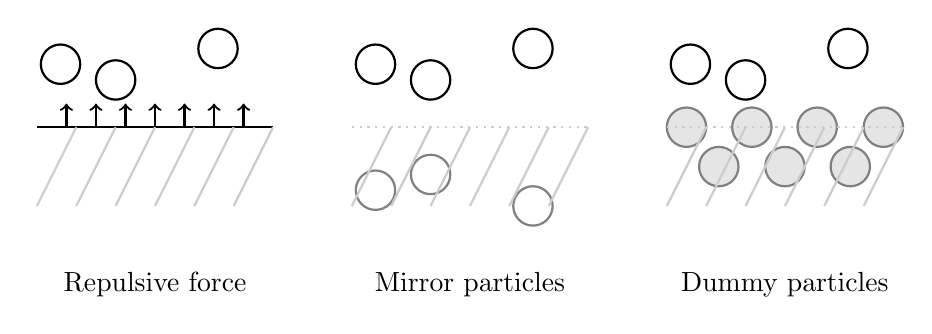
\begin{tikzpicture}[thick]
% Mathematical reflection
\draw (0.3,.8) circle (.25cm) node[pos=.5] (p0) {};
\draw (1,.6) circle (.25cm) node[pos=.5] (p1) {};
\draw (2.3,1) circle (.25cm) node[pos=.5] (p2) {};
\draw (0,0) -- (3,0);
\foreach \i in {1,...,6}{
	\draw[black!20] (.5*\i-.5,-1) -- (.5*\i,0);
}
% Forces
\foreach \i in {1,...,7}{
	\draw[->] (.375*\i,0) -- (.375*\i,.3);
}
\node at (1.5,-2) {Repulsive force};

% Mirror 
\draw (4.3,.8) circle (.25cm) node[pos=.5] (p0) {};
\draw (5,.6) circle (.25cm) node[pos=.5] (p1) {};
\draw (6.3,1) circle (.25cm) node[pos=.5] (p2) {};
\draw[black!50] (4.3,-.8) circle (.25cm) node[pos=.5] (mii1) {};
\draw[black!50] (5,-.6) circle (.25cm) node[pos=.5] (mii2) {};
\draw[black!50] (6.3,-1) circle (.25cm) node[pos=.5] (mii3) {};
\draw[black!20,dotted] (4,0) -- (7,0);
\foreach \i in {1,...,6}{
	\draw[black!20] (.5*\i-.5+4,-1) -- (.5*\i+4,0);
}
\node at (5.5,-2) {Mirror particles};

% Dummies
\draw[black!50,fill=black!10] (8.25,0) circle (.25cm) node[pos=.5] (d0) {};
\draw[black!50,fill=black!10] (9.08,0) circle (.25cm) node[pos=.5] (d1) {};
\draw[black!50,fill=black!10] (9.91,0) circle (.25cm) node[pos=.5] (d2) {};
\draw[black!50,fill=black!10] (10.75,0) circle (.25cm) node[pos=.5] (d3) {};
% second layer
\draw[black!50,fill=black!10] (8.66,-.5) circle (.25cm) node[pos=.5] (d4) {};
\draw[black!50,fill=black!10] (9.50,-.5) circle (.25cm) node[pos=.5] (d5) {};
\draw[black!50,fill=black!10] (10.33,-.5) circle (.25cm) node[pos=.5] (d6) {};
%\draw (1,-.25) circle (.25cm) node[pos=.5] (d4) {};
%normal parts
\draw (8.3,.8) circle (.25cm) node[pos=.5] (p0) {};
\draw (9,.6) circle (.25cm) node[pos=.5] (p1) {};
\draw (10.3,1) circle (.25cm) node[pos=.5] (p2) {};
\draw[dotted,black!20] (8,0) -- (11,0);
\foreach \i in {1,...,6}{
	\draw[black!20] (.5*\i-.5+8,-1) -- (.5*\i+8,0);
}
\node at (9.5,-2) {Dummy particles};
\end{tikzpicture}
\caption{Different boundaries condition methods}
\label{fig:SPH:boundaries}
\end{figure}

\subsubsection{Boundary conditions}
For this experiment, realistic boundaries conditions were needed. 
Several methods are possible with SPH and we focused on the main ones: the repulsive wall, the mirror particles \cite{libersky1991smooth} and the dummies particles implementation \cite{adami2012generalized}. 
Those boundaries conditions implementation are presented in figure~\ref{fig:SPH:boundaries}.

On our first implementation we used repulsive forces, but they imposed a lot of computation during the integration step and does not handle all the shape of boundaries easily. 

For the current implementation we used the dummies particles method.
This method is accurate and allows us to consider all the shape of boundaries.
The wall particles are just considered as normal particles, with specific equations, and their quantities are evolved during the run. 
The main difference is that their position does not evolve at the end of the step.
They are identified in the code with a specific type, provided during the data generation.\\ 

In this fluid flow example we were able to go up to a high number of particles with 2 or 3 dimensions. 
The handling of boundaries conditions added a pressure on the irregularity behavior. 

\subsection{SPH and gravitation}
%\subsection{Astrophysics: neutron stars coalescence}

The final aim of our tests is to simulate astrophysical events. 
We are interested in one of the most important event recently discovered. 
Last year the Laser Interferometer Gravitational Wave, LIGO, detected the first gravitational wave generated by binary neutron stars merging \cite{abbott2017gw170817} and also more complexes event with Binary Black Holes coalescence in \cite{abbott2017gw170814}.
We decided to conduct tests on Binary Neutron Star, BNS, coalescence. 
This problem represent all the aspect needed in our benchmark with the SPH method but also the self-gravitation and gravitation computation. 
In order to perform realistic simulations we consider two stars that are stable. 
We give details on the way to generate those data and the physics of the fusion itself. 
A lot of work have been involve in this understanding since it is quite out of the field of the primary researches. 

The generation of initial data for binary neutron star merging is quite complicated. 
THe first step is to generate the profile of mass regarding the radius of the star. 
This is made using the Lane-Emden equation. 
As those data are generated based on a grid with a fixed smoothing length in our case we need to add an extra step for relaxation. 
We used two relaxation methods with the Roche Lobe and Darwin problems. 
The last step before the merging is to positioned the stars and add the rotation velocity. 

\subsubsection{Solving Lane-Emden Equation}

In order to consider BNS we first consider two individual stars. 
The star is characterized by its radius and mass but also the density repartition inside.
Indeed, we have to determine the density function based on the radius. 
For this purpose we used the so called Land-Emden equation.\\

\todo{REFERENCE}
As we consider the star as a polytropic fluid, we use the equation of Lane-Emden which is a form of the Poisson equation: 

\begin{equation}\label{eq_LaneEmden}
  \frac{d^2\theta}{d \xi^2}+ \frac{2}{\xi}\frac{d\theta}{d\xi}+\theta^n = 0
\end{equation}

With $\xi$ and $\theta$ two dimensionless variables. 
There is only exact solutions for a polytropic index $n = 0.5$, $1$ and $2$.
In our work we use a polytropic index of $1$ which can correspond to a NS simulation.

For $n=1$ the solution of equation \ref{eq_LaneEmden} is: 

\begin{equation}
\theta(\xi)=\frac{sin(\xi)}{\xi}
\end{equation}

We note $\xi_1 = \pi$, the first value of $\xi$ with $\theta(\xi) = 0$.
$\theta(\xi)$ is also defined as: 
\begin{equation}
 \theta(\xi) = \Big(\frac{\rho(\xi)}{\rho_c}\Big)^{\frac{1}{n}}  = \frac{\rho(\xi)}{\rho_c}
\end{equation}

With $\rho_c$ the internal density of the star and $\rho$ the density at a determined radius. $\xi$ is defined as:  
$$ \xi = \sqrt{\frac{4\pi G}{K(n+1)}\rho_c^{(n-1)/n}} \times r = \sqrt{\frac{2\pi G}{K}}\times r = Ar\mbox{ (for } n=1 \mbox{ and } A=\sqrt{\frac{2\pi G}{K}} \mbox{)}$$

With $K$ a proportionality constant, $r$ the radius and $G$ the gravitational constant.

From the previous equations we can write the stellar radius $R$, the total radius of the star, as:
\begin{equation}
R = \sqrt{\frac{K(n+1)}{4\pi G}}\rho_c^{(1-n)/2}\xi_1 = \sqrt{ \frac{K}{2\pi G} } \times \xi_1 \mbox{ (for } n=1 \mbox{)}
\end{equation} 

We note that for $n=1$ the radius does not depend of the central density.

Here as an example we use dimensionless units as $G=R=M=1$ (for the other results we use CGS with $G = 6.674 \times 10^{-8} cm^3g^{-1}s^{-2}$) 
We can compute K as: 
\begin{equation}
\label{eq:constant}
K = \frac{R^2  2 \pi G}{\xi_1^2}
\end{equation}
%
\begin{table}[t!]
\centering
\begin{tabular}{|c|c|c|c|c|}
\hline
 & $\mbox{NS}_1$ & $\mbox{NS}_2$ & $\mbox{NS}_3$ & $\mbox{NS}_4$ \\ 
\hline 
Radius (cm) & $R=G=M=1$ & 1500000 & 1400000 & 960000 \\ 
\hline 
K & 0.636619 & 95598.00 & 83576.48 & 39156.94\\ 
\hline 
\end{tabular}
\caption{Examples of the proportionality constant $K$ regarding the star stellar radius $R$}
\label{tab:example_radius_k}
\end{table} 
Figure~\ref{tab:example_radius_k} give example of radius and the proportionality constant $K$.


Then we deduce the density function of $r$ as :

$$\rho(\xi) = \frac{sin(A\times r)}{A \times r} \times \rho_c \mbox{ with } A = \sqrt{\frac{2\pi G}{K}}
$$

As we know the total Mass $M$, the radius $R$ and the gravitational constant $G$ we can compute the central density as: 

$$ \rho_c = \frac{M A^3}{4 \pi (sin(AR)-ARcos(AR)) } $$

Then we normalize the results to fit $R = M = G = 1$: $K' = K/(R^2G) $, $m_i' = m_i/M $, $h_i' = h_i / R$, $\vec{x_i}' = \vec{x_i}/R$ 

\subsubsection{Generating Binary Neutron Stars initial data}
\label{sec:equi}

The initial data are based on a cubic lattice within a sphere of radius $R$.
The density function, based on radius, $\rho(\vec{r})$ is known using the result of the Lane-Emden equation ( we use polytropic index $n = 1$ here). 
The mass associate to each particle $i$ of the total $N$ particles: 

$$ m_i = \frac{\rho(\vec{r_i})}{n_r} \mbox{ with } n_r = \frac{3N}{4 \pi R^3}$$ 

The smoothing length is define constant and the same for all particles for all the simulation:

$$ h = \frac{1}{2}\sqrt{\frac{3N_N}{4\pi n}} $$ 

Here we choose $N_N$, the average number of neighbors, to be 100.

\subsubsection{Relaxation}
The last step is to perform a relaxation on the raw data. 
There is two methods we used: the Roche lobe and Darwin problems. 
In each of them we apply specific forces during a determined time for the particles to be stabilized. 

\paragraph{Roche lobe problem: }
The Roche Lobe version is used to simulate the halo around the stars which is shaped like a tear-drop. 
For this Hydrostatic Equilibrium Models we use a different equation of motion:

\begin{equation}
\frac{d\vec{v_i}}{dt} = \frac{\vec{F}_i^{Grav}}{m_i} + \frac{\vec{F}_i^{Hydro}}{m_i} + \vec{F}_i^{Roche} - \frac{\vec{v_i}}{t_{relax}}
\end{equation}

 
With $t_{relax} \leq t_{osc} \sim (G\rho)^{-1/2}$ and 
where $\vec{F}_i^{Roche}$ is:

$$\vec{F}_i^{Roche} = \mu (3+q) x_i \hat{\vec{x}} + \mu q y_i \hat{\vec{y}}-\mu z_i \hat{\vec{z}}$$ 

With $\mu$ to be determined (for us $\mu = 0.069$) and $q = \frac{M'}{M}=1$ as the two polytropes have the same total mass.
This is apply to each star to get the equilibrium and the simulate the tidal effect. 

\paragraph{Darwin problem: }
This is the way we use to generate the final simulation. 
The equation of motion for the relaxation is now: 
\begin{equation}
\label{eq:darwin}
\frac{d\vec{v_i}}{dt} = \frac{\vec{F}_i^{Grav}}{m_i} +\frac{\vec{F}_i^{Hydro}}{m_i} + \vec{F}_i^{Rot} - \frac{\vec{v_i}}{t_{relax}}
\end{equation}

With $t_{relax}$ same as before and $\vec{F}_{Rot}$ defined by:

\begin{equation}
\vec{F}_{Rot} = \Omega^2(x_i \vec{\hat{x}}+y_i\vec{\hat{y}})
\end{equation}

With $\Omega = \sqrt{\frac{G(M+M')}{a^3}}$, $L_z = Q_{zz}\Omega$ and $Q_{zz} = \sum_i(x_i^2+y_i^2)$. At $t=0$ we compute the total angular moment $L_z$ which stay constant.
Using it during the relaxation we can compute $\Omega$ as: $\Omega = \frac{L_z}{Q_{zz}}$ just by recomputing $Q_{zz}$.
Here the scheme is in $N^2$ but just for the relaxation step. 

For this relaxation we use two stars generated as before, applying equation of motion \ref{eq:darwin}.
Using $a$ as the distance between the two polytropes  (Here $a=2.9$ for $R=1$) and $\vec{\hat{x}}$ going for the center of the first to the second star, and $\vec{\hat{z}}$ is like the rotation vector.\\

After the generation we are able to perform BNS coalescence. 
This provides us a code using SPH, self-gravity and gravitation. 

\section{Conclusion}
The problem we presented in this part fulfill all the objectives for our metric. 
The computation wall is targeted via the physics and gravitation computation. 
The communication wall on the other hand is central regarding the exchanges needed for SPH and the fast multipole method. 
This problem is also very irregular for both cases. 
Indeed, the particles moves at every iteration without any prediction on their new position and data. 
In the same time the locality impose a very high level of irregularity to reach efficiently all the neighbors of a specific particle. 
This implies the usage of a tree data structure, the work of our two metrics can be apply in this context. 

As the SPH method is used in a large panel of fields from astrophysics to fluid mechanic, there are numerous related works. 
We can cite a code developed in the LANL, 2HOT \cite{warren20132hot} that introduced the Hashed Oct Tree structure used in our implementation. 
There is also GADGET-2 \cite{springel2005cosmological}, GIZMO \cite{hopkins2014gizmo} and the most recent publication is GASOLINE \cite{wadsley2017gasoline2} based on PKDGRAV, a specific tree+gravity implementation. 
Several implementations already implement GPU code and tree construction and traversal, one can cite GOTHIC \cite{miki2017gothic}, presenting gravitational tree code accelerated using the latest Fermi, Kepler and Maxwell architectures. But a lot of GPU accelerated work still focused on fluid problems and not on astrophysical problems  \cite{harada2007smoothed,crespo2011gpus}.
We also note that these implementations focus on SPH problems and does not provide a general purpose and multi-physics framework like we intent to provide through FleCSPH and FleCSI. 

Our implementation have not to be considered as a revolution for the SPH method itself, neither the use of accelerators. 
This study provide a code easy to use by domain scientists moving the complexity of distribution, load balancing and accelerator use to the back-end framework.
This tool will allows us to push forward and provide different type of accelerator in the future keeping a full transparency for the user. 
